\section{Designing generative models}
\label{subsec:design}
The steps to construct a generative model are best described by Box's loop~\cite{Blei2014} (\textbf{Figure~\ref{fig:overview}}). This procedure, originally proposed by George Box and colleagues~\cite{Box1976,Box1962}, traverses through the main steps of most applications: choosing a model (e.g., selecting the model type, the input covariates, and the distributions that describe these covariates), inferring parameter values (i.e., training), and criticizing the trained model (e.g., evaluating its accuracy on various tasks). After criticism, we return to the first step and iterate through the loop until we are ready to ``deploy'' our model.

An important consideration during model design is its \textit{interpretability} -- in the sense that its parameters will either be immediately useful (e.g., quantifying interactions between pairs of amino-acids~\cite{Riesselman2018}) or can be used in downstream analysis to extract knowledge (e.g., cell to cell similarity~\cite{Lopez2018}). It is often the case that there is a clear trade-off between model complexity and interpretability. Generative models that consist solely of linear operations (such as linear discriminant analysis or factor analysis) are easily interpretable since their parameters normally pertain directly to the input covariates (e.g., one coefficient per gene). This desirable property, however, comes at the cost of a limited ability to fit the data closely. Alternatively, models that use non-linear operations in neural networks (such as VAEs) are normally treated as black-boxes whose parameters are not interpretable. These models, however, usually provide a better fit to the observed data and an increased capacity to generalize upon it~(e.g.,~\cite{Riesselman2018}). The choice of the right trade-off therefore depends on the prospective uses of the model.

Next, we perform inference over the parameters (i.e., fit the model to data). Since exact inference is usually impossible for most types of generative models, one usually has to rely on approximate inference schemes. In this thesis, we focus on specific flavors of approximate inference that relies on neural networks as a way to achieve this. Our choice is motivated by a slew of theoretical and engineering advances that make the task of training generative models significantly more approachable than in the past.


Once the model is fit to the data, an important next step is model criticism. This is achieved by defining a set of attributes that we would like our model to have and a set of metrics to evaluate these attributes. A widely used attribute is the capacity to generalize, namely to properly describe data points that were not available during training. Relevant metrics include the likelihood of held out data points~\cite{wallach2009evaluation} or differences in summary statistics between observed and generated data~(Posterior Predictive Checks, [PPC] \cite{rubin1984bayesianly}). In the latter procedure, we sample random duplicates $\tilde{x}$ of a sample $x^*$ (often a group of samples) from the approximate posterior predictive distribution:
\begin{align}
    p(\tilde{x} \mid x^*) \approx \mathbb{E}_{q(z \mid  x^*)}p(\tilde{x} \mid z),
\end{align}
and compare this to the original data distribution. The comparison can be made by selecting key statistics for the data under scrutiny (e.g., comparing coefficient of variation of each gene in single-cell transcriptomics~\cite{Levitin2019}) and non-parametric tests. These metrics are especially suitable to evaluate Bayesian models but may not be defined for other DGMs.



\section{Encoding knowledge with likelihood-based generative models} 
\label{subsec:encoding_likelihood}
All the generative models in this thesis are explicitly defined via a likelihood function of the observed data. Our goal is to describe a distribution $p_{\theta}(x)$ from which each observation $x$ has been generated, where $\theta$ denotes the parameters of our model. A widely-used way of describing $p_\theta(x)$ with a Bayesian approach is not to model $x$ directly, but instead use an unobserved (latent) random variables $z$ as an intermediary. That is, to generate a new observations $x$ we first draw an intermediary value $z$ from a prior distribution $p_\theta(z)$ and then sample from a likelihood distribution $p_\theta(x\mid z)$~\cite{Wainwright:2008:GME:1498840.1498841}. There are two primary reasons for this modeling strategy. First, conditioning on $z$ allows us to decouple the contribution of individual entries in $x$ (e.g., positions along a sequence) to the overall likelihood of $x$. Since each entry in $x$ it assumed to be independent of all other entries when we condition on $z$, the inference of the parameters $\theta$ becomes substantially simpler. This simplification, for instance, aids DeepSequence to model high-order dependencies between amino acids, going beyond more traditional models~\cite{hopf2017mutation} that account only for pairwise interactions. Second, in many applications $z$ is of much lower dimension than $x$ and can thus provide a concise summary of the data. For instance, in scVI (the core work of this thesis), $z$ represents the cell state in a low dimensional space (typically set to less than $20$ dimensions) that summarizes the high dimensional observations of gene expression (usually thousands of genes). Note that using this property requires a mapping from each observation $x$ back to its representation $z$ in latent space. We discuss one way to achieve this in the next section.

With the use of intermediate variable $z$, the marginal probability (also termed the \emph{evidence}) of a given data set can be formally written by the a combination of the prior $p_\theta(z)$ and likelihood $p_\theta(x\mid z)$:
\begin{align}
\label{factorization}
\log p_\theta(x) = \log\left(\int \left[\prod_{j=1}^dp_\theta(x^j \mid z)\right]p_\theta(z)dz\right),
\end{align}
where $d$ is the dimension of each observation (e.g., length of sequence in DeepSequence) and $x^j$ denotes the $j-$th entry of observation $x$.
Notably, if the prior for $z$ is an isotropic Gaussian distribution:
\begin{align}
    z \sim \mathcal{N}(0, I)
\end{align}
and the likelihood for $x$ is a Gaussian with a linear link:
\begin{align}
    x \mid x \sim \mathcal{N}(u_j^Tz + v_j, \sigma_j^2),
\end{align}
then this formulation is a Bayesian version of principal components analysis (as we are specifying a prior for each entry of the principle components), otherwise known as factor analysis~\cite{Jolliffe1986}. 

While many practical applications indeed fix the prior to be an isotropic Gaussian,
the conditional distributions $p_\theta(x^j\mid z)$ usually come in other forms, which better reflect the nature of the data. For instance, scVI uses negative binomial - a distribution that adequately captures technical~\cite{love2014moderated} and biological~\cite{Grun2014a} noise in the observations of transcript counts. It also includes a possible addition of a zero inflation component to further account for sparseness~\cite{AutoZI}. Finally, scVI also supports the modeling of the conditional distribution $p_\theta(x \mid z, s)$ where $s$ denotes the batch information (treated as an observed random variable). This conditional VAE~\cite{Louizos2016} setting makes it particularly useful for removing of batch effects~\cite{Xu2019}. 

\section{Fitting a generative model using variational inference with neural networks}
\label{subsec:VI_deep}
Once we specified the form of the distributions (prior and likelihood) in our generative model, the inference task is two-fold. First, we would like to find a set of parameters $\theta$ that maximizes the evidence for the data (Equation~\eqref{factorization}). In parallel, for a complete model we would also like to infer the \textit{posterior} distribution $p_\theta(z \mid x)$, which provides a way to represent our observations in the low dimensional latent space. While the parameters $\theta$ can be computed precisely for a restricted choice of distributions (e.g., in factor analysis~\cite{Jolliffe1986} or other cases where the prior is conjugate to the likelihood), exact inference is intractable for most real world applications. Indeed, evaluating the evidence requires integration over the latent variable $z$, which may take exponential time to compute or for which a closed form is not available~\cite{jordan1999introduction}. The same caveat also applies to evaluating the posterior distribution. To see this, recall that Bayes rule entails that:
\begin{align}
\label{eq:Bayesrule}
     p_\theta(z \mid x) = \frac{p_\theta(x \mid z)p_\theta(z)}{p_\theta(x)}.
\end{align}
The numerator in this equation can be readily computed in most applications since the prior and likelihood come with a pre-specified closed form density. However, the denominator is the intractable evidence term.


The main idea behind variational inference is the realization that the problems of maximizing $p_{\theta}(x)$ and approximating $p_{\theta}(z \mid x)$ are very much related. As one way to see this, assume that our goal is to find a distribution $q_{\phi}(z_i)$ (also known as \textit{variational posterior}) that, for a given $\theta$ best approximates the posterior. In other words, for every observation $x_i$, its variational posterior $q_{\phi}(z_i)$ should be as similar as possible to the actual posterior $p_{\theta}(z \mid x_i)$. Because the evidence decomposes across datapoints, we present here the derivation for the evidence of a unique observation. Using Bayes rule, we have for each value of~$z$: 
\begin{align}
    \log p_\theta(x) &= \log \frac{p_\theta(x \mid z)p_\theta(z)}{p_\theta(z \mid x)}.  \label{eq:logBayes} 
\end{align}
We can therefore take expectation of both sides of Equation~\eqref{eq:logBayes} with respect to $q_\phi(z)$ to decompose the evidence as:
\begin{align}
    \log p_\theta(x) &= \mathbb{E}_{q_\phi(z)} \log \frac{p_\theta(x \mid z)p_\theta(z)}{p_\theta(z \mid x)}\\
    &= \mathbb{E}_{q_\phi(z)} \log \left(\frac{p_\theta(x \mid z)p_\theta(z)}{q_\phi(z)}. \frac{q_\phi(z)}{p_\theta(z \mid x)}\right) \\
    &= \mathbb{E}_{q_\phi(z)}\log \frac{p_\theta(x \mid z)p_\theta(z)}{q_\phi(z)} + \mathbb{E}_{q_\phi(z)}\log \frac{q_\phi(z)}{p_\theta(z \mid x)}  \\
    &= \underbrace{\mathbb{E}_{q_\phi(z)} \log \frac{p_\theta(x \mid z)p_\theta(z)}{q_\phi(z)}}_{\text{Evidence lower bound (ELBO)}} +\underbrace{ \kl{q_\phi(z)}{p_\theta(z \mid x)}}_{\text{Variational gap}}, \label{eqn:ELBO_decomp}
\end{align}
where $\Delta_\textrm{KL}$ denotes the Kullback-Leibler (KL) divergence, a notion of similarity between probability distribution. In Equation~\eqref{eqn:ELBO_decomp}, the variational gap quantifies how well $q_\phi(z)$ approximates the posterior and is always positive because that is the KL divergence between two distributions. Consequently, the ELBO is indeed a valid lower bound on the evidence.

Variational inference avoids the intractability of the evidence by maximizing the ELBO, which helps address both of our inference problems. 
The ELBO includes two sets of parameters. The first set $\theta$ controls the generative model and the second set $\phi$ controls the variational approximation to the posterior. Maximizing the ELBO with respect to $\phi$ for a fixed $\theta$ yields an approximation to the posterior $p_\theta(z \mid x)$ and the ELBO approaches the marginal probability $p_{\theta}(x)$. In practice, however, we do not have $\theta$ and the optimization procedure includes assignments of values to both the generative model parameters $\theta$ and the variational posterior parameters $\phi$ so as to maximize the respective ELBO. 


While the ELBO optimization problem is well-studied~\cite{Blei2017}, recent advances in the field provide an effective way to address it using stochastic optimization~\cite{Hoffman2013} as well as neural networks, leading to substantial increase in scalability and (for large enough data sets) accuracy. 
A notable way to achieve this is with \textit{variational autoencoders}~\cite{Kingma2014,Rezende2014}.

\section{Variational auto-encoders}\label{box:VAE}
VAEs provide a way for explicitly representing and then jointly inferring both the variational posterior and the generative model.  A standard VAE model consists of two components (Figure~\ref{vae_fig}): an \textit{encoder} neural network that maps any given point in the observation space ($x_i$) to its corresponding location in latent space ($z_i$). The mapping is done by setting the parameters of the variational posterior $q_{\phi}(z_i)$ for any given observation $x_i$ through a function $f_\phi$ represented by the encoder network. In this notation, $\phi$ refers to the weights of the encoder network. For example, with a Gaussian variational approximation $q_{\phi}(z_i) = \textrm{Normal}\left(\mu_i, \textrm{diag}(v_i)\right)$, we have $(\mu_i, v_i) = f_\phi(x_i)$. Because we can compute $\mu_i$ and $v_i$ with a neural network, we do not need to store these values in memory (by opposition to classical variational inference). Notably, because we can obtain the values of the variational parameters at any observation $x$ (using the encoder network), we refer to the variational distribution as $q_\phi(z \mid x)$. The second component is a \textit{decoder} neural network that maps any given point in the latent space ($z$) to the space of observations ($x$). The mapping is done by setting the parameters of the generative model $p_{\theta}(x \mid z)$. 
\begin{figure}\centering
    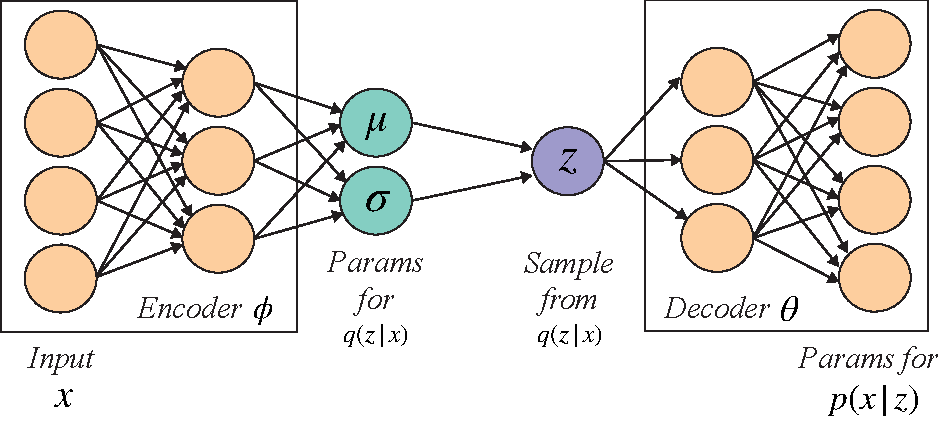
\includegraphics[width=0.6\textwidth]{review/figures/vae.pdf}\\
      \caption{\label{vae_fig}Computational Schematics of the VAE}
\end{figure}
      
A rich literature surrounds the VAE, both in applications and methods development. For instance, the VAE has been applied to image generation~\cite{Gregor2015}, object segmentation with partial observation~\cite{Sohn2015} and astronomy~\cite{AAAI1714765}. Others have focused on improving parts of the framework such as a different (possibly tighter) lower bound~\cite{Li2016,Burda2016}, better posterior approximation~\cite{Kingma2016a}, more flexible choices of distributions~\cite{Ruiz2016} and richer family of graphical models~\cite{NIPS2016_6379}.


